\documentclass[ignorenonframetext,]{beamer}
\usetheme{Rochester}
\usecolortheme{beaver}
\usepackage{amssymb,amsmath}
\usepackage{ifxetex,ifluatex}
\usepackage{fixltx2e} % provides \textsubscript
\ifxetex
  \usepackage{fontspec,xltxtra,xunicode}
  \defaultfontfeatures{Mapping=tex-text,Scale=MatchLowercase}
\else
  \ifluatex
    \usepackage{fontspec}
    \defaultfontfeatures{Mapping=tex-text,Scale=MatchLowercase}
  \else
    \usepackage[utf8]{inputenc}
  \fi
\fi
\usepackage{biblatex}
\bibliography{bibdatabase}
\usepackage{graphicx}
\usepackage{helvet}
\usepackage{hyperref}
\usepackage[portuguese]{babel}
\makeatletter
\def\ScaleIfNeededV{%
  \ifdim\Gin@nat@width>0.9\linewidth
    0.9\linewidth
  \else
    \Gin@nat@width
  \fi
}
\def\ScaleIfNeededH{%
  \ifdim\Gin@nat@height>0.9\textheight
    0.9\textheight
  \else
    \Gin@nat@height
  \fi
}
\makeatother
\let\Oldincludegraphics\includegraphics
\renewcommand{\includegraphics}[2][]{\Oldincludegraphics[width=\ScaleIfNeededV,height=\ScaleIfNeededH,keepaspectratio]{#2}}


% Comment these out if you don't want a slide with just the
% part/section/subsection/subsubsection title:
\AtBeginPart{
  \let\insertpartnumber\relax
  \let\partname\relax
  \frame{\partpage}
}
\AtBeginSection{
  \let\insertsectionnumber\relax
  \let\sectionname\relax
  \frame{\sectionpage}
}
\AtBeginSubsection{
  \let\insertsubsectionnumber\relax
  \let\subsectionname\relax
  \frame{\subsectionpage}
}

\setlength{\parindent}{0pt}
\setlength{\parskip}{6pt plus 2pt minus 1pt}
\setlength{\emergencystretch}{3em}  % prevent overfull lines
\setcounter{secnumdepth}{0}
\beamertemplatenavigationsymbolsempty
\title[Tese]{Uma abordagem mecânico-estatística de dois tópicos de interesse em
       finanças, economia e sociologia.}
\author{Rafael S. Calsaverini}
\date{\today}

\begin{document}
\frame{\titlepage}

\begin{frame}
\tableofcontents[hideallsubsections]
\end{frame}

\begin{frame}



\end{frame}

\section{Parte 1: Teoria de dependência estatística, Cópulas e teoria de
informação}

\begin{frame}\frametitle{Parte 1: Teoria de dependência estatística,
Cópulas e teoria de informação}

\begin{itemize}
\itemsep1pt\parskip0pt\parsep0pt
\item
  \href{http://iopscience.iop.org/0295-5075/88/6/68003?ejredirect=migration}{Artigo}
  R. S. Calsaverini and R. Vicente. An information-theoretic approach to
  statistical dependence: Copula information.\emph{Europhys. Lett.} 88
  68003, 2009.
\item
  URL:
  http://iopscience.iop.org/0295-5075/88/6/68003?ejredirect=migration
\item
  \href{https://github.com/rcalsaverini/Thesis}{Repositório git da
  tese}: http://github.com/rcalsaverini/Thesis
\end{itemize}

\end{frame}

\begin{frame}\frametitle{Dependência estatística}

\begin{itemize}
\itemsep1pt\parskip0pt\parsep0pt
\item
  Independência estatística: $P(x,y) = P(x)P(y)$, ou:
  \[P(x\vert y) = P(x)\]
\item
  Dependência completa: $P(x\vert y) = \delta(x - F(y))$
\item
  Definição informal: quanta informação uma variável oferece sobre o
  valor de outra.
\item
  Como medir dependência?
\item
  É possível separar informação idiossincrática sobre cada variável da
  informação a respeito de sua dependência?
\end{itemize}

\end{frame}

\begin{frame}\frametitle{Correlação}

\begin{itemize}
\itemsep1pt\parskip0pt\parsep0pt
\item
  Módulo usualmente empregado como medida de dependência estatística.
  \[\vert \mathrm{Corr}(X,Y)\vert  = \left\vert  \frac{E[XY] - E[X]E[Y]}{\sigma[X]\sigma[Y]}\right\vert \]
\item
  Correlação é problemática:

  \begin{itemize}
  \itemsep1pt\parskip0pt\parsep0pt
  \item
    $\mathrm{Corr}(X,Y) \ne \mathrm{Corr}(f(X), g(Y)) $, em geral;
  \item
    $\mathrm{Corr}(X,Y) = 0$ não implica que $X$ e $Y$ sejam
    independentes;
  \item
    $\mathrm{Corr}(X,Y) = 1$ não implica que $X$ e $Y$ tenham
    dependência perfeita.
  \end{itemize}
\end{itemize}

\end{frame}

\begin{frame}\frametitle{Medidas de dependência}

\begin{itemize}
\itemsep1pt\parskip0pt\parsep0pt
\item
  Desideratos para uma boa medida de dependência
  \footnote{A. Renyi. \textit{Acta. Math. Acad. Sci. Hungar.}, 10:441–451, 1959;}

  \begin{itemize}
  \itemsep1pt\parskip0pt\parsep0pt
  \item
    $M[X,Y]$ é um funcional da distribuição conjunta;
  \item
    $M[X,Y] = M[Y,X]$;
  \item
    $M[X,Y]$ é mínimo $\Leftrightarrow$ $X$ e $Y$ independentes;
  \item
    $M[X,Y]$ é máximo $\Leftrightarrow$
    $P(X\vert Y) = \delta(X - f(Y))$;
  \item
    $M[X,Y] = M[g(X), f(Y)]$ $\forall g, f$ monotônicas
  \item
    Se $X,Y \thicksim \mathrm{Normal}(\sigma_X, \sigma_Y, \rho)$, então
    $M[X,Y] = f(\rho)$
  \end{itemize}
\end{itemize}

\end{frame}

\begin{frame}\frametitle{Medida de dependência}

\begin{itemize}
\itemsep1pt\parskip0pt\parsep0pt
\item
  Exemplos:

  \begin{itemize}
  \itemsep1pt\parskip0pt\parsep0pt
  \item
    $\tau$ de Kendall
    \[\small\tau = \mathrm{Prob}\left[(X - X')(Y-Y') > 0\right] - \mathrm{Prob}\left[(X - X')(Y-Y') < 0\right]\]
  \item
    $\rho$ de Spearman.
    \[\rho = \mathrm{Corr}(\mathrm{rank}(X), \mathrm{rank}(Y))\]
  \end{itemize}
\end{itemize}

\end{frame}

\begin{frame}\frametitle{Informação Mútua}

\begin{itemize}
\item
  Definição

  \[I(X,Y) = \int \mathrm{d}x\mathrm{d}y\; p(x,y) \log\frac{p(x,y)}{p(x)p(y)}\]

  \begin{enumerate}
  \def\labelenumi{\arabic{enumi}.}
  \itemsep1pt\parskip0pt\parsep0pt
  \item
    ``Distância''
    \footnote{divergência de Kullback-Leibler: $\int p(x)\log\frac{p(x)}{q(x)} \;\mathrm{d}x$}
    entre a distribuição conjunta e a variedade de distribuições
    fatoráveis
  \item
    Valor esperado da divergência KL entre $p(x)$ e $p(x\vert Y = y)$
  \item
    Valor esperado da redução na entropia de $X$ ao se obter o valor de
    $Y$
  \end{enumerate}
\item
  Para qualquer distribuição:
  $I(X,Y) \ge -\frac{1}{2} \log(1 - \mathrm{Corr}(X,Y)^2)$
\end{itemize}

\end{frame}

\begin{frame}\frametitle{Cópulas - Teorema de Sklar}

Para toda distribuição cumulativa conjunta contínua de duas variáveis
$F_{X,Y}(x,y)$, com distribuições cumulativas $F_X(x)$ e $F_Y(y)$,
existe uma função cópula única $C(u, v)$ tal que:
$F_{X,Y}(x,y) = C(F_X(x), F_Y(y))$

\begin{itemize}
\itemsep1pt\parskip0pt\parsep0pt
\item
  Exemplos

  \begin{itemize}
  \itemsep1pt\parskip0pt\parsep0pt
  \item
    Arquimedianas: $C(u,v) = \psi^{-1}(\psi(u) + \psi(v))$
  \item
    Normal:
    $N_{\rho}(u,v) = \frac{1}{2\pi\sqrt{1 - \rho^2}}\int_{-\infty}^{\Phi^{-1}(u)} \int_{-\infty}^{\Phi^{-1}(v)} \mathrm{d} u \mathrm{d} v\; e^{-\frac{u^2 + v^2 - 2uv\rho}{2(1-\rho^2)}}$
  \end{itemize}
\item
  Densidade de cópula:

  \begin{itemize}
  \itemsep1pt\parskip0pt\parsep0pt
  \item
    $c(u,v)=\frac{\partial^2 C}{\partial u\partial v}$
  \item
    $p_{XY}(x,y)=c(F_X(x),F_Y(y))p_X(x)p_Y(y)$
  \end{itemize}
\end{itemize}

\end{frame}

\begin{frame}\frametitle{Medidas de dependência revisitadas}

\begin{itemize}
\itemsep1pt\parskip0pt\parsep0pt
\item
  Desideratos para uma boa medida de dependência:

  \begin{itemize}
  \itemsep1pt\parskip0pt\parsep0pt
  \item
    $M[X,Y]$ é um funcional da cópula, e não depende das distribuições
    marginais;
  \item
    $M[X,Y]$ é mínimo se $C(u,v) = uv$;
  \item
    $M[X,Y]$ é máximo se $C(u,v) = \max(0,u+v-1)$ ou $C(u,v)=\min(u,v)$,
    chamadas cópulas de Frechet-Hoeffding;
  \item
    Se $C(u,v) = N_\rho(u,v)$, então $M[X,Y] = f(\rho)$
  \end{itemize}
\item
  As exigências de (Renyi, 1959) são consequencia imediata das
  exigências acima.
\end{itemize}

\end{frame}

\begin{frame}\frametitle{Medidas de dependência e cópulas}

\begin{itemize}
\item
  $\tau$ de Kendall: $\tau=4 \int_0^1\int_0^1 C(u,v) \mathrm{d}C(u,v)-1$
\item
  $\rho$ de Spearman:
  $\rho_{S}=12 \int_0^1\int_0^1 \left[C(u,v) - uv\right] \mathrm{d}u \mathrm{d}v$
\item
  Informação Mútua:

  \begin{itemize}
  \itemsep1pt\parskip0pt\parsep0pt
  \item
    Entropia da cópula:
    \[I(X,Y) = \int \int \mathrm{d} u \mathrm{d} v \; c(u,v) \log c(u,v)  = - S[c] \ge 0\]
  \item
    para a cópula normal: $I(X,Y) = -\frac{1}{2} \log(1 - \rho^2)$
  \item
    Decomposição: $H[X, Y] = H[X] + H[Y] + H[\mathrm{copula}]$
  \item
    Cópula gaussiana maximiza entropia para dada correlação linear.
  \end{itemize}
\end{itemize}

\end{frame}

\begin{frame}\frametitle{Problemas com a Correlação}
    \begin{columns}
        \column{.5\textwidth}
          \begin{figure}[htbp]
	    \Oldincludegraphics[width=1.15\textwidth]{./figs/mutinfo2.png}
	  \end{figure}
        \column{.5\textwidth}
          \begin{minipage}[c][.6\textheight][c]{\linewidth}
	    \begin{itemize}
	    \itemsep1pt\parskip0pt\parsep0pt
	    \item
	      $\mathrm{Corr}(X,Y)$ depende explicitamente das distribuições
	      marginais
	    \item
	      $\mathrm{Corr}(X,Y)$ vs. $\rho$: correlação não é um bom estimador do
	      parâmetro $\rho$.
	    \item
	      $\mathrm{Corr}(X,Y)$ pode subestimar grosseiramente a dependência.
	    \end{itemize}
          \end{minipage}
      \end{columns}
\end{frame}


\begin{frame}\frametitle{Cópulas esféricas e elipticas}

\begin{itemize}
\itemsep1pt\parskip0pt\parsep0pt
\item
  Distribuição esféricas e elípticas:

  \begin{itemize}
  \itemsep1pt\parskip0pt\parsep0pt
  \item
    Distribuição $p(\vec{x})$ é esférica se
    $E\left[ e^{i\vec{k}\cdot\vec{x}}\right] = \psi\left(\vert k\vert ^2/2\right)$
  \item
    Distribuição $p(\vec{y})$ é elíptica se
    $E\left[ e^{i\vec{k}\cdot\vec{y}}\right] = \psi\left(\frac{1}{2}\vec{k}\Sigma^T \vec{k}\right)$
  \item
    $\vec{X} \thicksim$ distribuição esférica
    $\Rightarrow \vec{Y} = A\vec{X} \thicksim$ distribuição elíptica,
  \end{itemize}
\item
  Proposição: Se $C(u,v \vert  \Sigma)$ é cópula elíptica derivada da
  cópula esférica $C(u,v)$, então:
  \[I[C(u,v\vert \Sigma)] = I_{0}(\Sigma) + I[C(u,v)]\] onde
  $I_{0}(\Sigma) = -\frac{1}{2}\log\Sigma$ é a informação mútua de uma
  cópula normal com matriz de correlação $\Sigma$.
\end{itemize}

\end{frame}

\begin{frame}\frametitle{Excesso de Informação Mútua - teste de
normalidade na dependência}

\begin{itemize}
\itemsep1pt\parskip0pt\parsep0pt
\item
  Parte gaussiana da dependência é associada a dependência linear.
\item
  $I[X,Y] \ge -\frac{1}{2}\log(1 - \rho^2)$ para distribuições
  elípticas.
\item
  $\tau$ de Kendall para distribuições elípticas
  $\rho = \sin\left(\frac{\pi\tau}{2}\right)$
\item
  Algoritmo de Kraskov-Stogbauer-Grassberger
  \footnote{Kraskov et al. Phys. Rev. E, 69:066138, 2004}
\end{itemize}

\end{frame}

\begin{frame}\frametitle{Excesso de Informação Mútua - teste de
normalidade na dependência}

\begin{figure}[htbp]
\centering
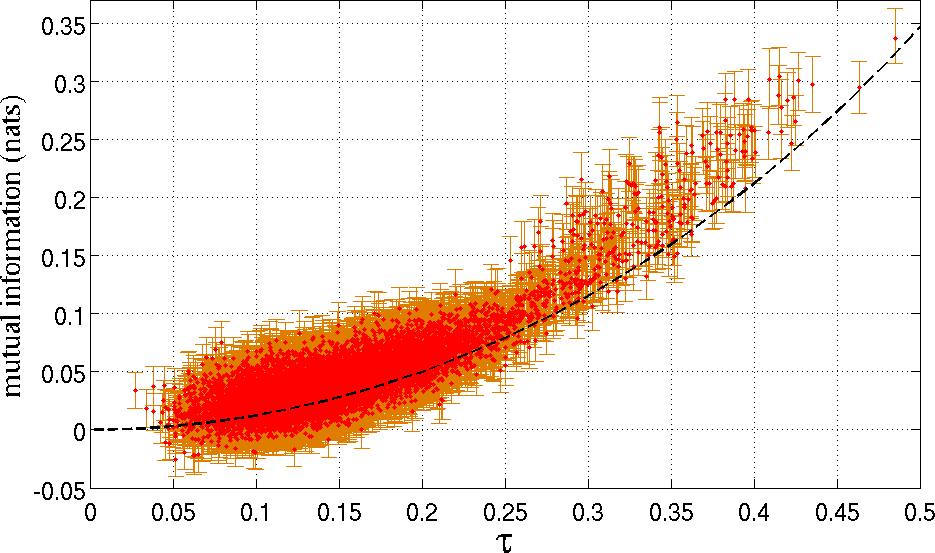
\includegraphics{./figs/MIvsrho_tau_final2.png}
\caption{Informação mútua vs. $\tau$ para pares de séries temporais de
log-retornos de abertura vs.~fechamento para ações que compões o
S\&P500. Intervalos de confiança de 90\% via bootstrap.}
\end{figure}

\end{frame}

\begin{frame}\frametitle{Excesso de Informação Mútua - teste de
normalidade na dependência}

\begin{figure}[htbp]
\centering
\Oldincludegraphics[width=0.85\textwidth]{./figs/locohimi.png}
\caption{Seleção de pares de ações com baixa correlação e grande excesso
de informação mútua.}
\end{figure}

\end{frame}

\begin{frame}\frametitle{Excesso de Informação Mútua - teste de
normalidade na dependência}

\begin{figure}[htbp]
\centering
\Oldincludegraphics[width=0.85\textwidth]{./figs/gausscompat.png}
\caption{Seleção de pares de ações compatíveis com uma cópula normal.}
\end{figure}

\end{frame}

\begin{frame}\frametitle{Cópula t - ajuste}

\begin{itemize}
\itemsep1pt\parskip0pt\parsep0pt
\item
  Método de ``moment matching'' via $\tau$ de Kendall e informação mútua
\item
  Distribuição t de Student $\to$ Cópula t
  \[p_{t}(x,y\mid  \rho, \nu) = \frac{\Gamma(1+\frac{\nu}{2})}{\Gamma(\frac{\nu}{2}){\pi\nu\sqrt{1-\rho^2}}}\left[1+ \frac{x^2+ y^2 - 2\rho xy}{(1-\rho^2)\nu}\right]^{-(1+\frac{\nu}{2})}\]
\item
  fat tails, tail dependency, $t(\rho, \nu) \to \mathrm{Normal}(\rho)$
  quando $\nu\to\infty$
\item
  Cópula $t$:
  \[C_{T}(u,v\vert \nu, \rho) = \int_{-\infty}^{t_\nu^{-1}(u)} \int_{-\infty}^{t_\nu^{-1}(v)} \mathrm{d} x \mathrm{d}y \; p_{t}(x, y \mid \rho, \nu)\]
\end{itemize}

\end{frame}

\begin{frame}\frametitle{Cópula t - ajuste}

\begin{itemize}
\itemsep1pt\parskip0pt\parsep0pt
\item
  Se $\vec{x} \sim t(\rho, \nu)$, então
  $I(x_1, x_2, \ldots, x_n) = n H_{1}(\nu) - H_n(\nu)$
\item
  $H_{n}(\nu)$ pode ser calculada usando um truque similar ao truque de
  réplicas
  $\log(x) = \lim_{a\to\infty}\frac{\partial}{\partial a} (x^a)$
\item
  Informação mútua:
  $I(\nu) = 2\log\left(\sqrt{\frac{\nu}{2\pi}}B\left(\frac{\nu}{2},\frac{1}{2}\right) \right) - \frac{2+\nu}{\nu} + (1+\nu)\left[ \psi \left(\frac{\nu+1}{2}\right) - \psi \left(\frac{\nu}{2}\right) \right]$
\item
  Ajuste:

  \begin{itemize}
  \itemsep1pt\parskip0pt\parsep0pt
  \item
    $\rho$ é ajustado medindo $\tau$
  \item
    $\nu$ é ajustado medindo $I(X,Y)$
  \end{itemize}
\item
  Simulação:

  \begin{itemize}
  \itemsep1pt\parskip0pt\parsep0pt
  \item
    excesso de informação mútua com relação à distribuição normal vs.
    $\nu$
  \item
    $I_\text{excess}$ independe de $\rho$
  \end{itemize}
\end{itemize}

\end{frame}

\begin{frame}\frametitle{Cópula t - ajuste}

\begin{figure}[htbp]
\centering
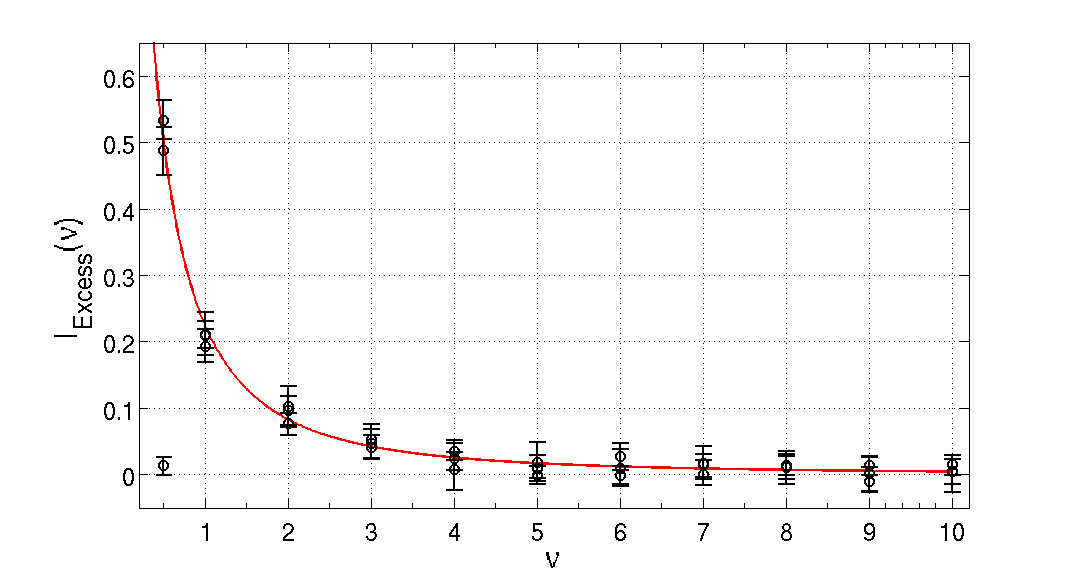
\includegraphics{./figs/I_Excess.png}
\caption{Cada círculo corresponde a uma amostragem de 20 valores
sampleados de uma distribuição $t$ para vários valores de $\nu$ e $\rho$
conhecidos. Intervalo de confiança de 90\% via bootstrap.}
\end{figure}

\end{frame}

\begin{frame}\frametitle{Considerações finais}

\begin{itemize}
\itemsep1pt\parskip0pt\parsep0pt
\item
  Decomposição da dependência entre parte linear e não linear
\item
  Teste de normalidade \emph{da dependência}
\item
  Ajuste de cópulas empíricas a dados experimentais
\item
  Detecção de dependência não-trivial em séries temporais financeiras
\item
  Problemas com inferência de dependência baseada apenas correlação
\end{itemize}

\end{frame}

\section{Parte 2: Um modelo para emergência de autoridade em sociedades
humanas}

\begin{frame}\frametitle{Comportamento social igualitário
vs.~hierárquico}

\begin{itemize}
\itemsep1pt\parskip0pt\parsep0pt
\item
  Organização social - igualitária vs.~autoritária

  \begin{itemize}
  \itemsep1pt\parskip0pt\parsep0pt
  \item
    Grandes primatas (Chimpanzés, Bonobos, Gorilas)
  \item
    Diversidade de comportamentos social humano
  \item
    Origem da diversidade: ecológica vs.~cultural.
  \end{itemize}
\end{itemize}

\end{frame}

\begin{frame}\frametitle{Evidências empíricas}

\begin{itemize}
\itemsep1pt\parskip0pt\parsep0pt
\item
  Evolução do comportamento social humano (``u-shaped
  evolution'')\footnote{Knauft et al. Current Anthropology, 32:391–428, 1991.; Joyce Marcus. Annu. Rev. Anthropol, 37:25166, 2008}:
\end{itemize}

\begin{figure}[htbp]
\centering
\Oldincludegraphics[height=0.5\textheight]{./figs/ushaped.png}
\caption{Evolução do comportamento social humano}
\end{figure}

\end{frame}

\begin{frame}\frametitle{Evidências empíricas}

\begin{itemize}
\item
  Ancestrais hierárquicos, paleolítico igualitário, neolítico
  hierárquico
\item
  Humanos modernos - relação entre tamanho de grupo e formas de
  organização
  social\footnote{Currie et al. Nature, 467(7317):801–804, Oct. 2010}.
\item
  Hipótese do cérebro social

  \begin{itemize}
  \itemsep1pt\parskip0pt\parsep0pt
  \item
    Capacidade cognitiva vs.~tamanho de grupo. Número de Dunbar
    \textasciitilde{} 150.
  \item
    Pressão seletiva sobre capacidade cognitiva
    social\footnote{T Sawaguchi and H Kudo. Primates, 31:283–90, 1990; Robin Dunbar. Journal of Human Evolution, 20:469–93, 1992}.
  \end{itemize}
\end{itemize}

\end{frame}

\begin{frame}\frametitle{Evidências empíricas}

\begin{figure}[htbp]
\centering
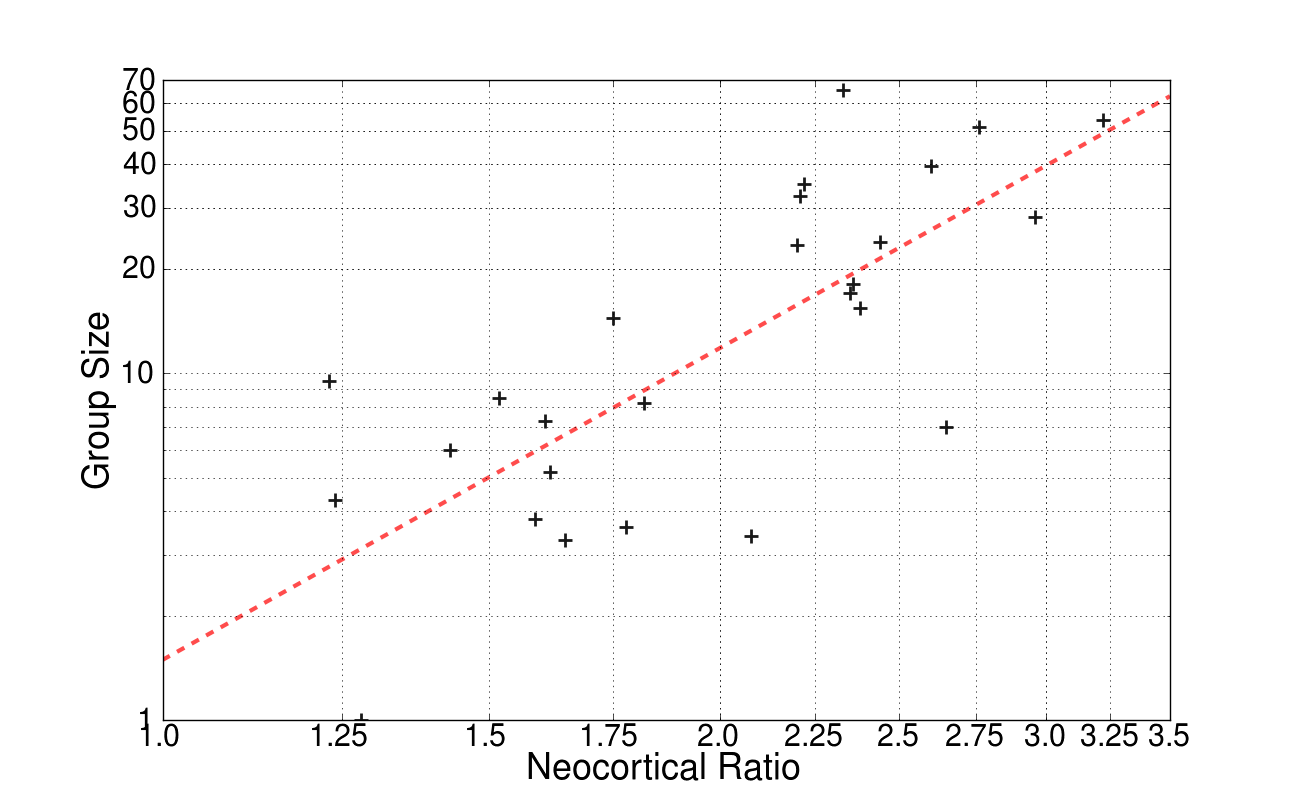
\includegraphics{./figs/dunbar.png}
\caption{Razão neocortical vs.~tamanho típico de grupo para diferentes
espécies de primatas. Adaptado de (Dunbar, 1992)}
\end{figure}

\end{frame}

\begin{frame}\frametitle{Evidências empíricas}

\begin{itemize}
\itemsep1pt\parskip0pt\parsep0pt
\item
  Reverse dominance
  theory\footnote{Boehm et al. Current Anthropology, 34 (3):227–254, 1993; Boehm. Hierarchy in the Forest: The Evolution of Egalitarian Behavior. Harvard University Press, 2001.}

  \begin{itemize}
  \itemsep1pt\parskip0pt\parsep0pt
  \item
    Manutenção de estruturas igualitárias em grupos de individuos com
    comportamento de dominância.
  \item
    Reversão da dominância: candidatos a líder tem mecanismos de
    ascenção limitados por outros membros do grupo.
  \item
    Observado em estudos de agrupamentos humanos de caçadores-coletores.
  \end{itemize}
\end{itemize}

\end{frame}

\begin{frame}\frametitle{Modelo baseado em agentes}

\begin{itemize}
\itemsep1pt\parskip0pt\parsep0pt
\item
  Grupo de $n$ agentes com capacidade cognitiva limitada.
\item
  Mapa mental das relações sociais do grupo, codificado em um grafo.

  \begin{itemize}
  \itemsep1pt\parskip0pt\parsep0pt
  \item
    Aresta conectada: relação conhecida. Aresta ausente: relação
    desconhecida.
  \end{itemize}
\item
  Agente aprende nova informação através de observação e aprendizado
  social.
\item
  Aprendizado e manutenção de informação social é custoso (limitação
  cognitiva).
\item
  Agente deve balancear custos:

  \begin{itemize}
  \itemsep1pt\parskip0pt\parsep0pt
  \item
    Custo cognitivo de obter, armazenar e processar informação social:
    $C_{c} \propto n_{e}$
  \item
    Custo Social de cometer erros de julgamento em situações sociais:
    $C_{s} \propto \frac{2}{n(n-1)}\sum_{i<j}L_{ij}$
  \end{itemize}
\end{itemize}

\end{frame}

\begin{frame}\frametitle{Agentes isolados}

\begin{itemize}
\item
  Variáveis dinâmicas do agente $k$:
  \[M^{k}_{ij} = \begin{cases} 1  & \text{se $i$ e $j$ estão ligados no grafo de $k$} \\\\  0  & \text{outro caso}   \end{cases}\]
\item
  Custo total do agente $k$:
  $C(M^k, \alpha) = \frac{n_{\text{edges}}(M^k)}{n(n-1)/2} + \alpha \bar{L}(M^k)$
\item
  Modelo de máxima entropia (vínculo: grafo conexo):
  \[P(M \vert  \alpha, \beta) = \frac{q(M^k)}{Z(\alpha, \beta)} e^{-\beta C(M^k, \alpha)}\]
\item
  Interpretação dos parâmetros

  \begin{itemize}
  \item
    $\alpha$ - importância relativa entre os custos, proxy para
    capacidade cognitiva.
  \item
    $\beta$ - intensidade de flutuações, pressão para otimização do
    custo total
  \end{itemize}
\end{itemize}

\end{frame}

\begin{frame}\frametitle{Minimização do custo ($\beta \to \infty$)}
    \begin{columns}
        \column{.5\textwidth}
	  \begin{itemize}
	  \itemsep1pt\parskip0pt\parsep0pt
	  \item
	    $\alpha \gg 1$:
	  \end{itemize}

	  \begin{figure}[htbp]
	  \centering
	  \Oldincludegraphics[height=0.7\textheight]{./figs/fullyconnected.png}
	  \caption{Grafo totalmente conectado}
	  \end{figure}
        \column{.5\textwidth}
	  \begin{itemize}
	  \itemsep1pt\parskip0pt\parsep0pt
	  \item
	    $\alpha \ll 1$:
	  \end{itemize}

	  \begin{figure}[htbp]
	  \centering
	  \Oldincludegraphics[height=0.7\textheight]{./figs/starGraph.png}
	  \caption{Grafo estrela}
	  \end{figure}
      \end{columns}
\end{frame}


\begin{frame}\frametitle{Simulações - corte do diagrama de fases}

\begin{figure}[htbp]
\centering
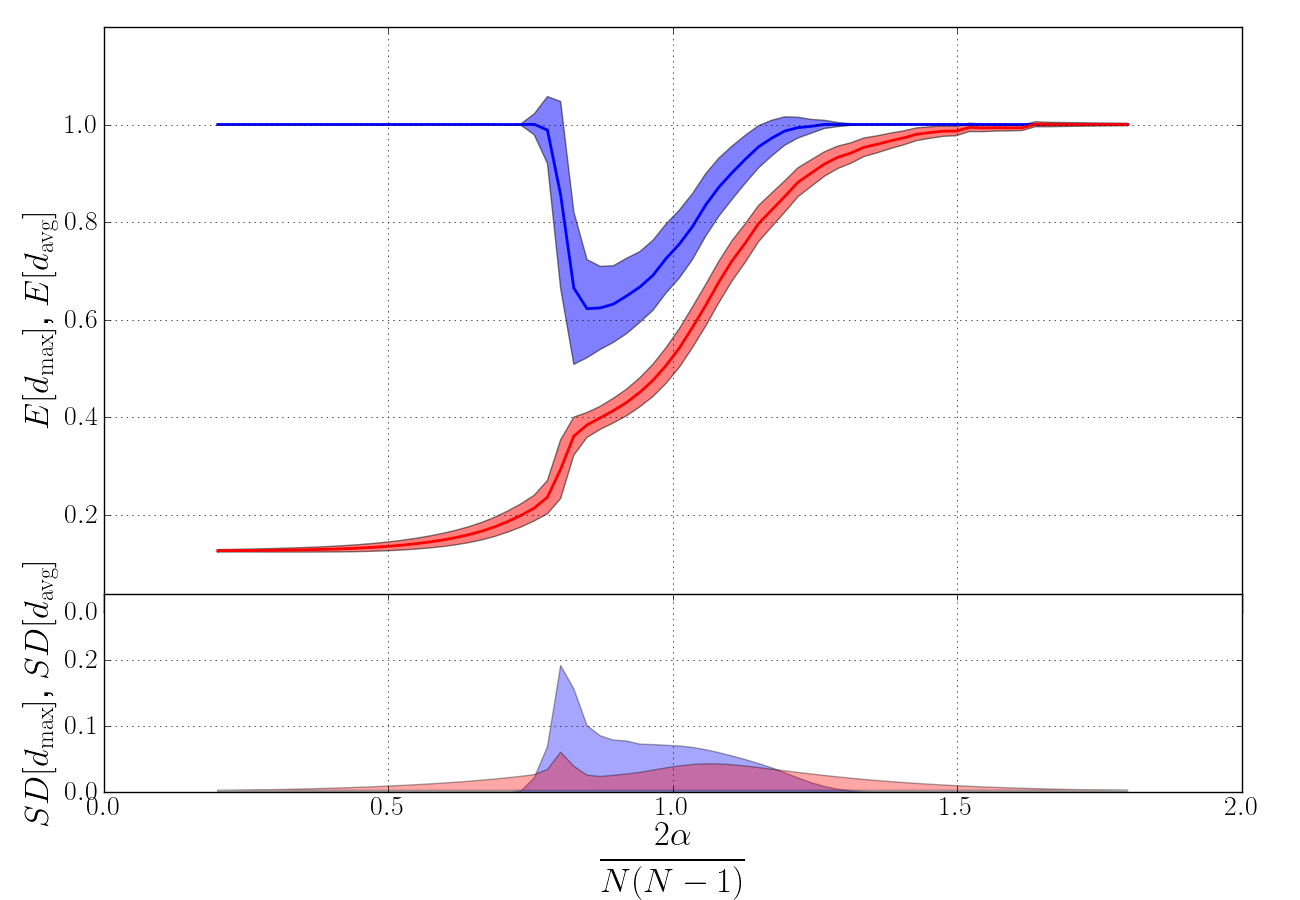
\includegraphics{./figs/cut.png}
\end{figure}

\end{frame}

\begin{frame}\frametitle{Simulações - corte do diagrama de fases}

\begin{figure}[htbp]
\centering
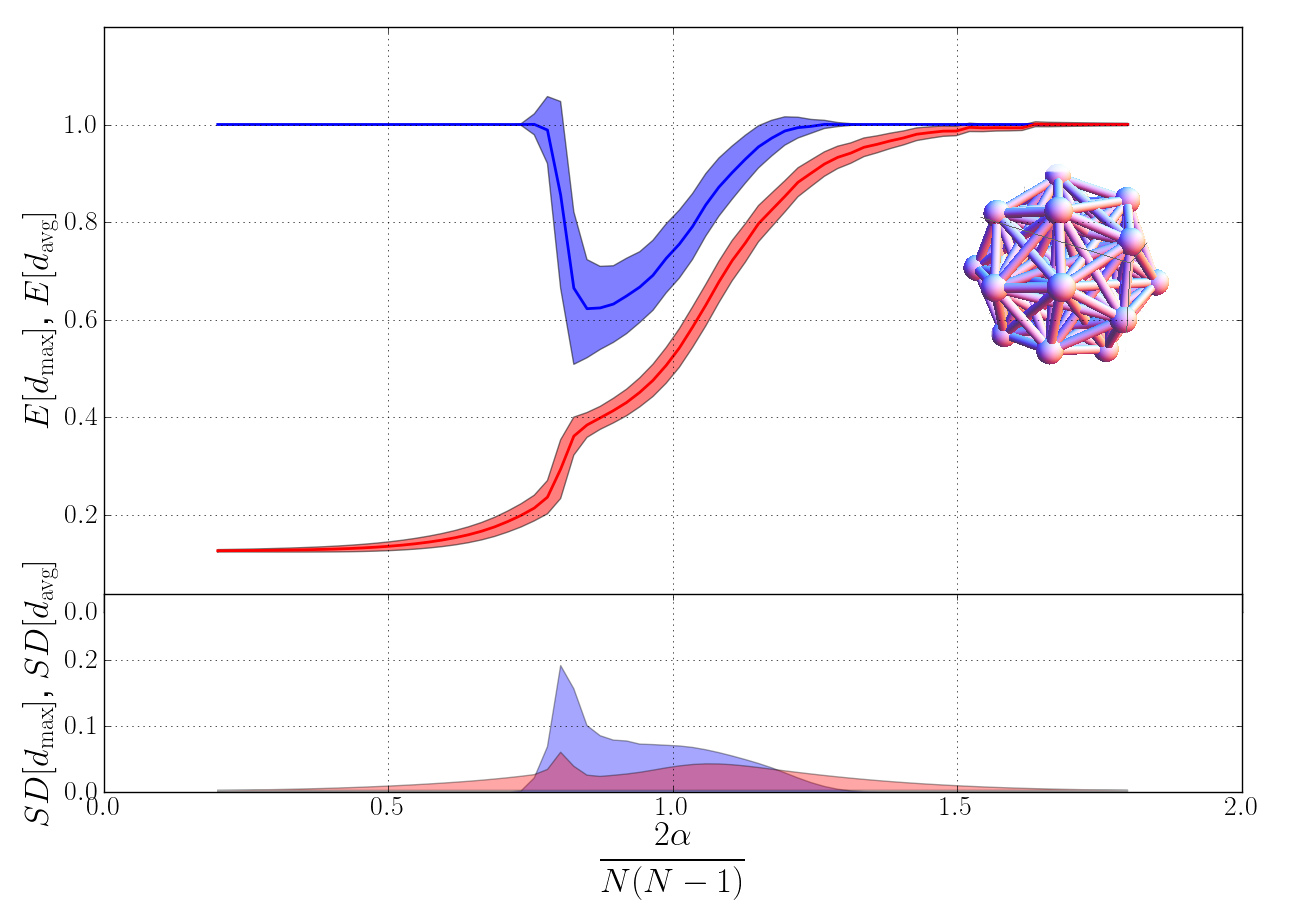
\includegraphics{./figs/cutfull.png}
\end{figure}

\end{frame}

\begin{frame}\frametitle{Simulações - corte do diagrama de fases}

\begin{figure}[htbp]
\centering
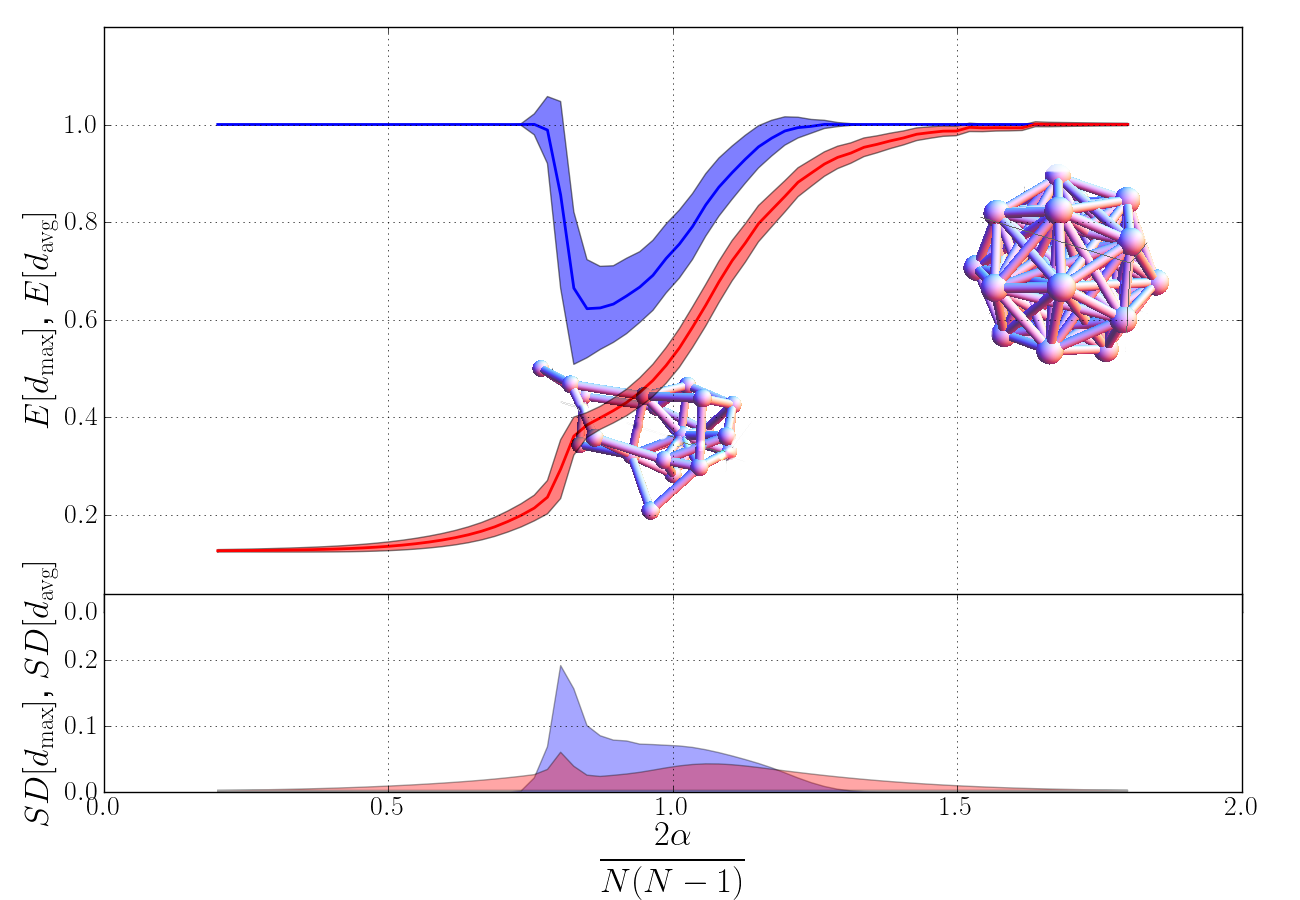
\includegraphics{./figs/cutstruggle.png}
\end{figure}

\end{frame}

\begin{frame}\frametitle{Simulações - corte do diagrama de fases}

\begin{figure}[htbp]
\centering
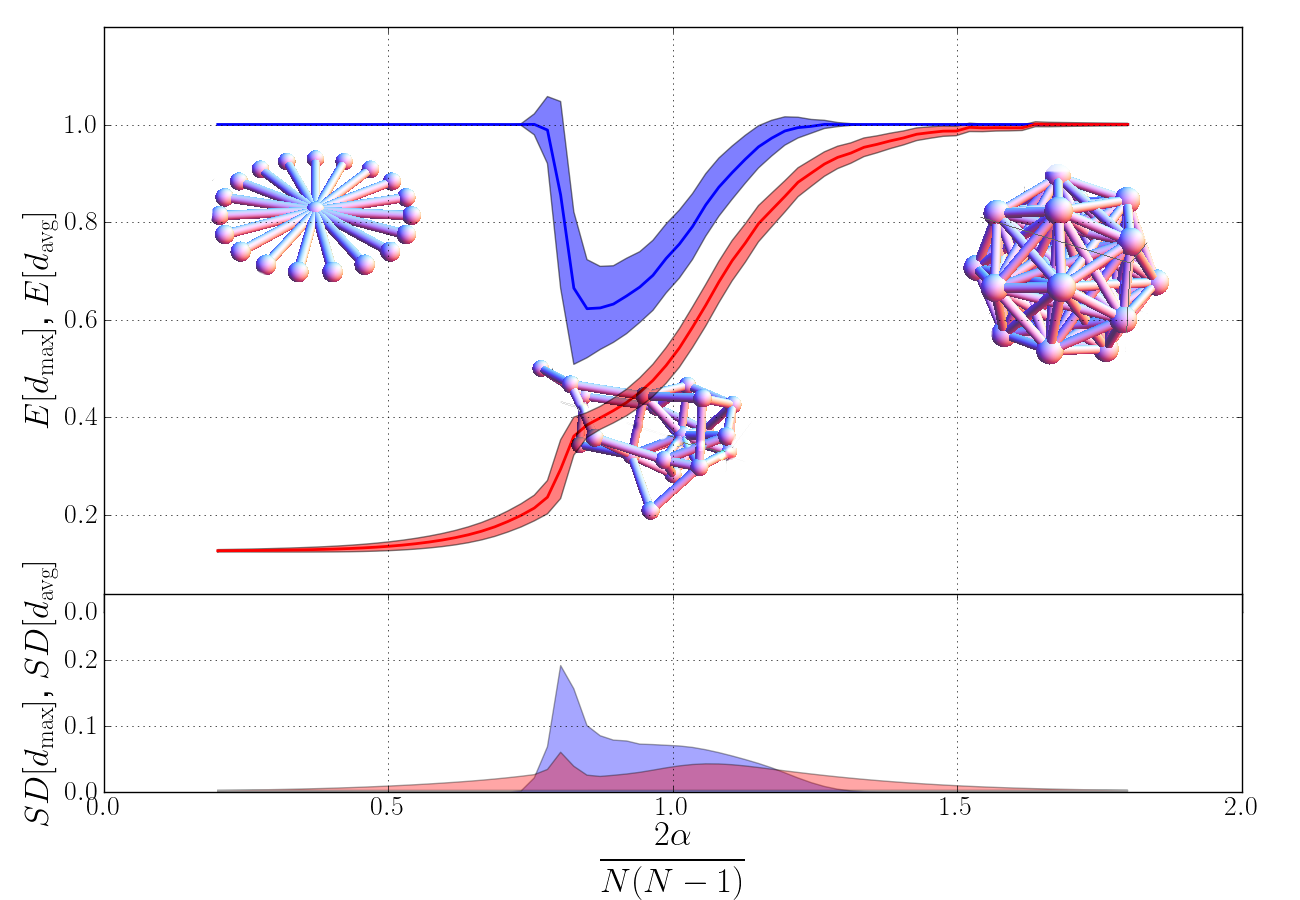
\includegraphics{./figs/cutstar.png}
\end{figure}

\end{frame}

\begin{frame}\frametitle{Simulações - diagrama de fases}

\begin{figure}[htbp]
\centering
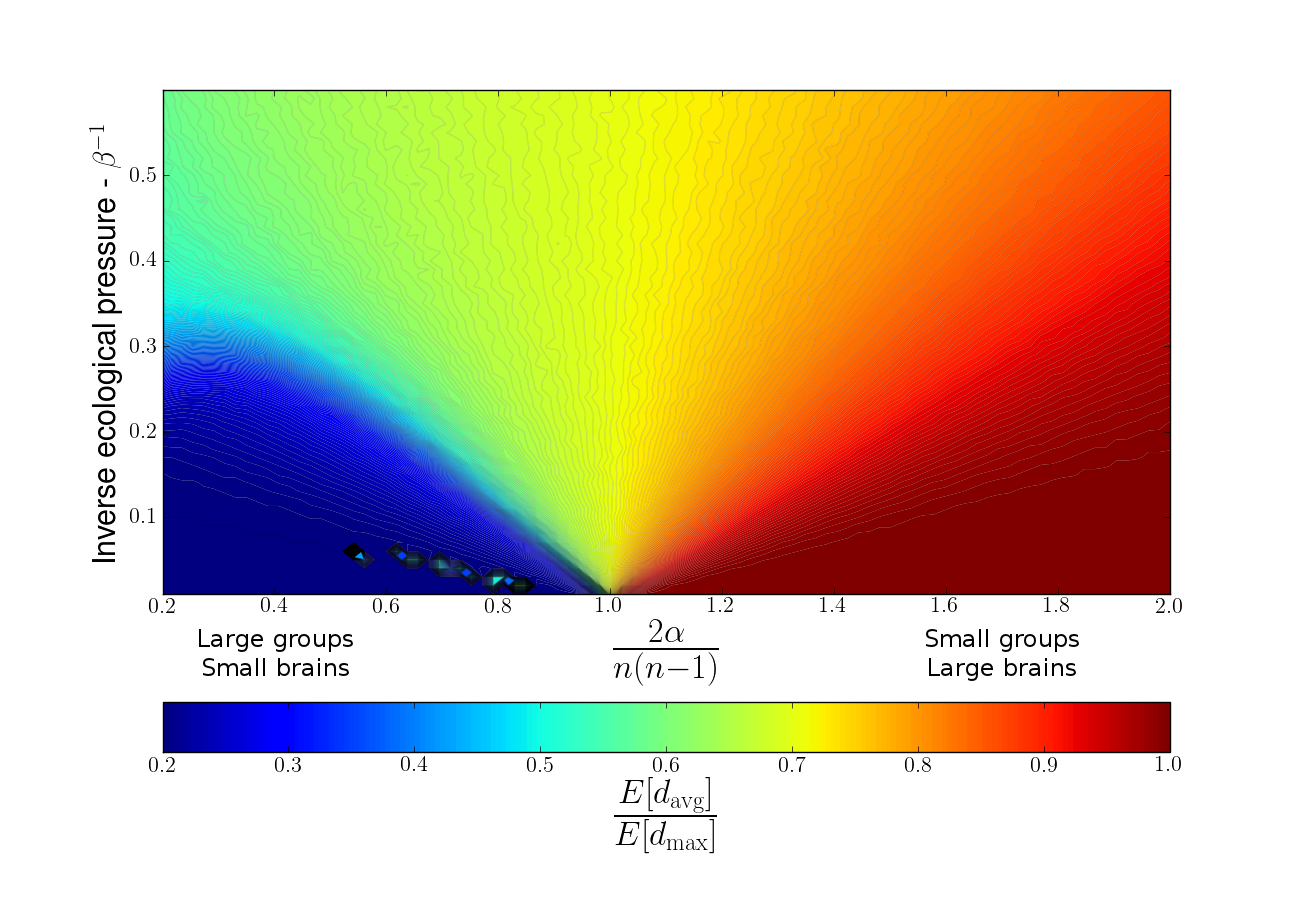
\includegraphics{./figs/phasediagram.png}
\end{figure}

\end{frame}

\begin{frame}\frametitle{Simulações - $\alpha$ crítico vs. $\beta$}

\begin{figure}[htbp]
\centering
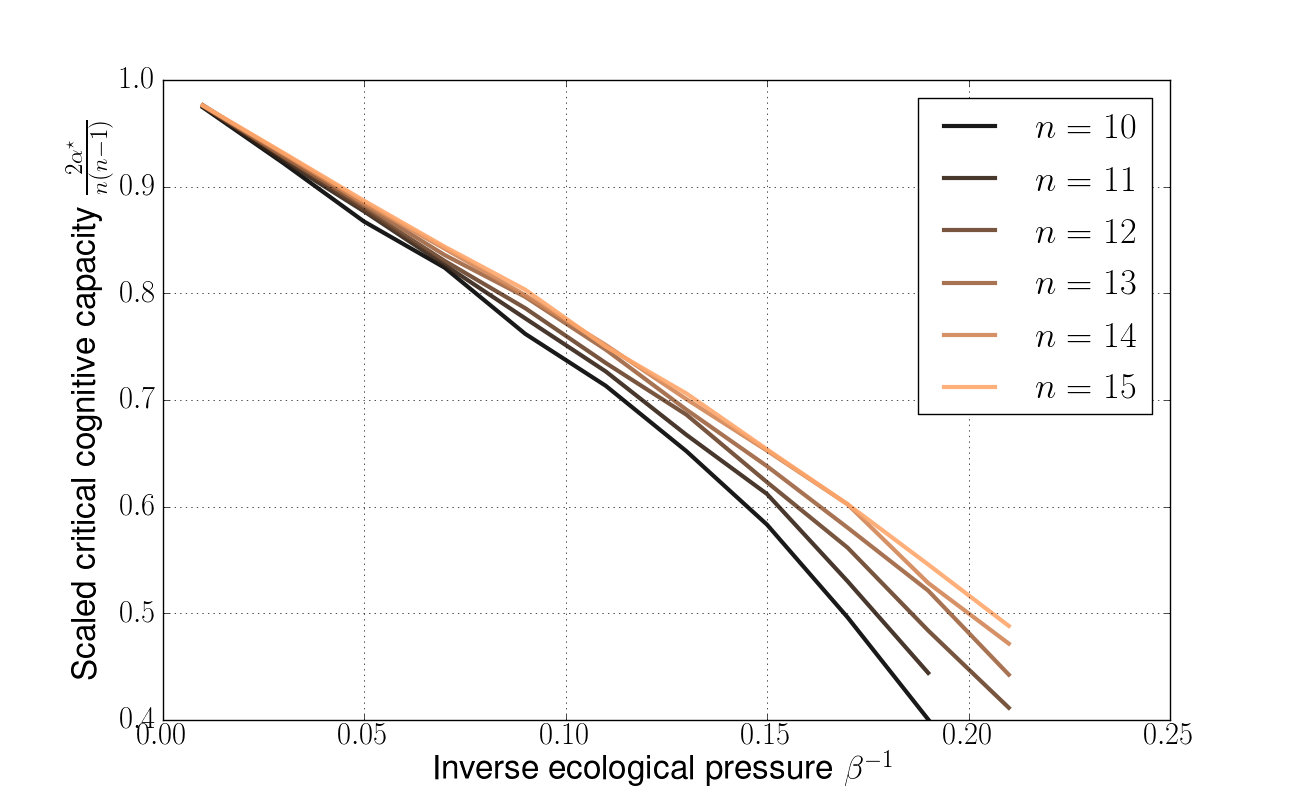
\includegraphics{./figs/critical.png}
\end{figure}

\end{frame}

\begin{frame}\frametitle{Simulações - taxa de aceitação do Monte Carlo}

\begin{figure}[htbp]
\centering
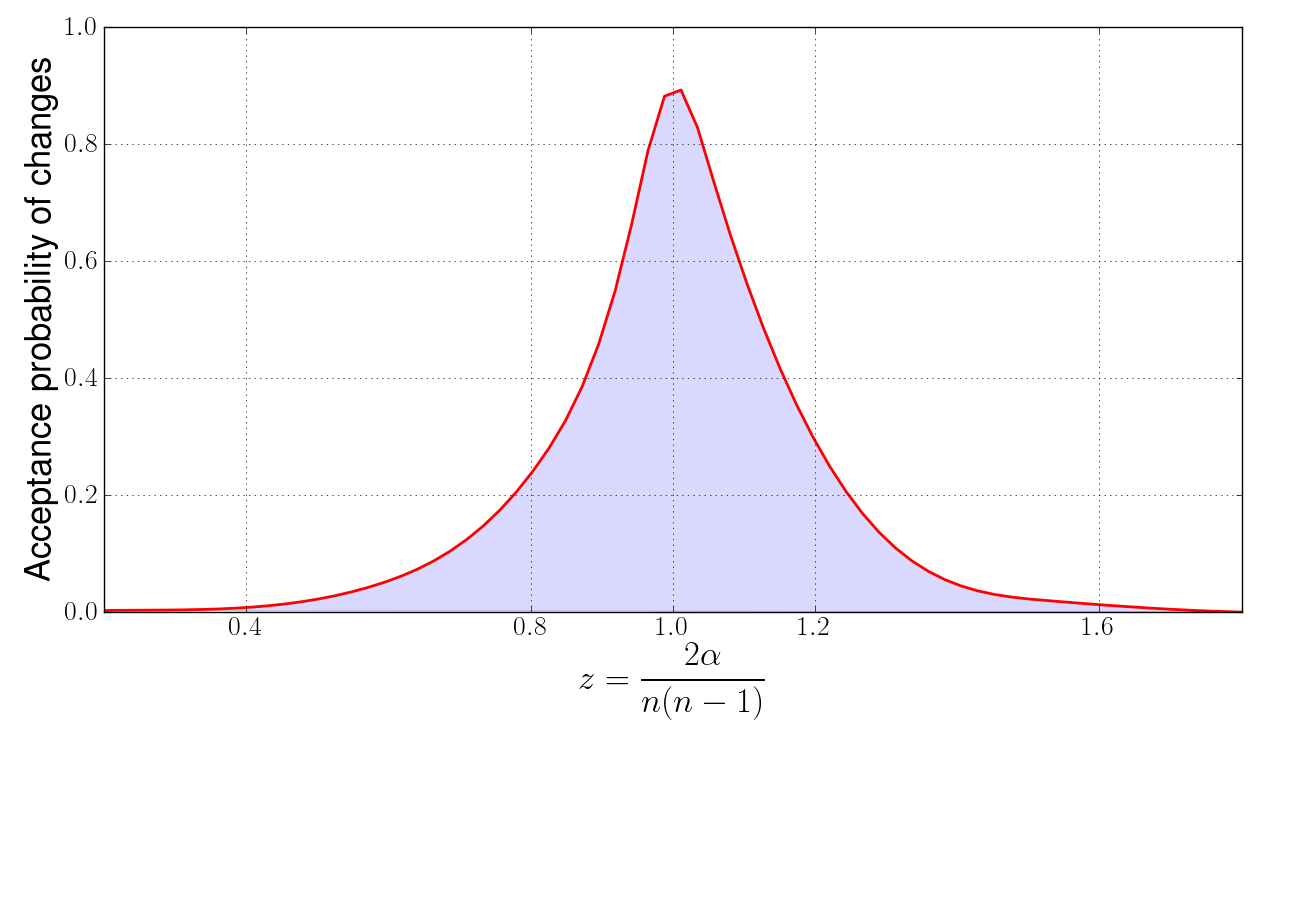
\includegraphics{./figs/acceptrate.png}
\end{figure}

\end{frame}

\begin{frame}\frametitle{Agentes em interação}

\begin{itemize}
\itemsep1pt\parskip0pt\parsep0pt
\item
  Agentes podem interagir através de ``fofoca''
\item
  A simulação inclui agora $n$ grafos com $n(n-1)/2$ arestas cada
\item
  A cada passo de Monte Carlo:

  \begin{itemize}
  \itemsep1pt\parskip0pt\parsep0pt
  \item
    com probabilidade $1-g$, há proposta de troca aleatória de uma
    aresta,
  \item
    com probabilidade $g$, é proposta a mesma aresta do grafo de outro
    agente,
  \item
    a alteração proposta é aceita com probabilidade
    $e^{-\beta \Delta H}$
  \end{itemize}
\item
  Equivale a introduzir um termo de interação $M^k_{ij} M^l_{ij}$ no
  custo total
\end{itemize}

\end{frame}

\begin{frame}\frametitle{Simulações - muitos agentes}

\begin{figure}[htbp]
\centering
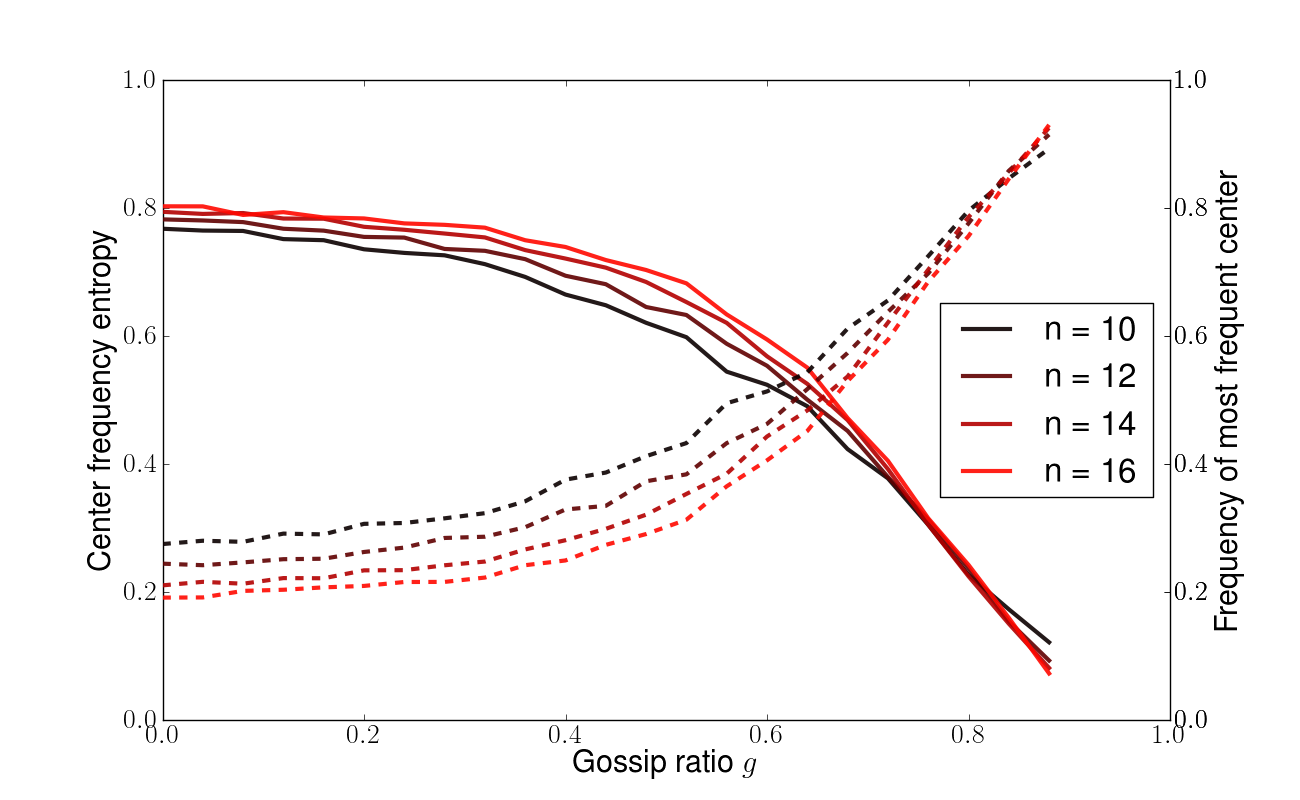
\includegraphics{./figs/gossip.png}
\end{figure}

\end{frame}

\begin{frame}\frametitle{Sumário e Interpretação}

\begin{itemize}
\itemsep1pt\parskip0pt\parsep0pt
\item
  Parâmetros de controle: $\alpha$, $\beta$ e $g$

  \begin{itemize}
  \item
    $\alpha$ grande: Situação social simétrica + reverse dominance
    theory, sistema igualitário
  \item
    $\alpha$ intemediário: Grandes flutuações, situação social fluida,
    concentração de centralidade, dominância temporária, \emph{primus
    inter pares}
  \item
    $\alpha$ pequeno, $g$ grande: Quebra de simetria, todos os grafos
    centrados no mesmo agente, sistema hierárquico
  \end{itemize}
\end{itemize}

\end{frame}

\begin{frame}\frametitle{Conclusões}

\begin{itemize}
\itemsep1pt\parskip0pt\parsep0pt
\item
  Foi construído um modelo de agentes para tentar elucidar o problema da
  diversidade do comportamento social humano.
\item
  O modelo apresenta três parâmetros, associados (1) à capacidade
  cognitiva da espécie, (2) às pressões ecológicas e sociais por
  eficiência na minimização de custos e (3) ao nível de comunicação
  entre os agentes a respeito de relações sociais.
\item
  Três fases de interesse emergem nesse modelo que, à luz de outras
  evidências, podem ser interpretadas como formas distintas de
  organização social - uma igualitária, uma socialmente fluida, com
  constantes flutuações, e uma hierárquica.
\end{itemize}

\end{frame}

\begin{frame}\frametitle{Conclusões}

\begin{itemize}
\itemsep1pt\parskip0pt\parsep0pt
\item
  A existência de limitações cognitivas é suficiente, no modelo, para
  causar uma quebra de simetria que está na raiz da fase hierárquica.
\item
  O modelo corrobora informações empíricas:

  \begin{itemize}
  \itemsep1pt\parskip0pt\parsep0pt
  \item
    a respeito da relação entre número de agentes e forma de organização
    social (Currie et al, Kennet \& Winterhalder);
  \item
    a respeito da relação entre pressões ecológicas e sociais nas formas
    de organização social (Earle, Summers).
  \end{itemize}
\item
  A comparação com dados empíricos etnográficos é útil na avaliação da
  utilidade analítica desse modelo.
\end{itemize}

\end{frame}

\begin{frame}\frametitle{Bibliografia}

\begin{itemize}
\itemsep1pt\parskip0pt\parsep0pt
\item
  A. Renyi. On measures of dependence. \emph{Acta. Math. Acad. Sci.
  Hungar.} , 10:441--451, 1959.
\item
  Alexander Kraskov, Harald Stögbauer, and Peter Grassberger. Estimating
  mutual information. \emph{Phys. Rev.~E}, 69:066138, 2004.
\item
  Bruce M. Knauft et al. Violence and sociality in human evolution.
  \emph{Current Anthropology}, 32:391--428, 1991.
\item
  Joyce Marcus. The archeological evidence for social evolution.
  \emph{Annu. Rev.~Anthropol.}, 37:25166, 2008.
\item
  Thomas E. Currie et al. Rise and fall of political complexity in
  island south-east asia and the pacific. Nature, 467(7317):801--804,
  Oct. 2010.
\item
  T Sawaguchi and H Kudo. Neocortical development and social structure
  in primates. \emph{Primates}, pages 283--90, 1990
\end{itemize}

\end{frame}

\begin{frame}\frametitle{Bibliografia}

\begin{itemize}
\itemsep1pt\parskip0pt\parsep0pt
\item
  Robin Dunbar. Neocortex size as a constraint on group size in
  primates. \emph{Journal of Human Evolution}, 20:469--93, 1992.
\item
  Christopher Boehm et al. Egalitarian behavior and reverse dominance
  hierarchy {[}and comments and reply{]}. \emph{Current Anthropology},
  34(3):pp.~227--254, 1993. ISSN 00113204.
\item
  C Boehm. \emph{Hierarchy in the Forest: The Evolution of Egalitarian
  Behavior}. Harvard University Press, 2001. ISBN 9780674006911.
\item
  Douglas J. Kennett and Bruce Winterhalder. \emph{Islands of Inquiry:
  Colonisation, seafaring and the archaeology of maritime landscapes,
  chapter Demographic expansion, despotism and the colonisation of East
  and South Polynesia}, pages 87--96. In Clark et al. {[}40{]}, 2008.
\end{itemize}

\end{frame}

\begin{frame}\frametitle{Bibliografia}

\begin{itemize}
\itemsep1pt\parskip0pt\parsep0pt
\item
  T.K. Earle. \emph{How Chiefs Come to Power: The Political Economy in
  Prehistory}. Antropology. Political science. Stanford University
  Press, 1997
\item
  K. Summers. The evolutionary ecology of despotism. \emph{Evolution and
  Human Behavior}, 26(1):106--135, 2005.
\end{itemize}

\end{frame}

\printbibliography

\end{document}
